\documentclass[]{article}
\usepackage{lmodern}
\usepackage{amssymb,amsmath}
\usepackage{ifxetex,ifluatex}
\usepackage{fixltx2e} % provides \textsubscript
\ifnum 0\ifxetex 1\fi\ifluatex 1\fi=0 % if pdftex
  \usepackage[T1]{fontenc}
  \usepackage[utf8]{inputenc}
\else % if luatex or xelatex
  \ifxetex
    \usepackage{mathspec}
  \else
    \usepackage{fontspec}
  \fi
  \defaultfontfeatures{Ligatures=TeX,Scale=MatchLowercase}
\fi
% use upquote if available, for straight quotes in verbatim environments
\IfFileExists{upquote.sty}{\usepackage{upquote}}{}
% use microtype if available
\IfFileExists{microtype.sty}{%
\usepackage{microtype}
\UseMicrotypeSet[protrusion]{basicmath} % disable protrusion for tt fonts
}{}
\usepackage[margin=1in]{geometry}
\usepackage{hyperref}
\hypersetup{unicode=true,
            pdftitle={Final Report},
            pdfauthor={Nikki Johnson, Molly Hischke, Collin Brehmer, and Kyle Hancock},
            pdfborder={0 0 0},
            breaklinks=true}
\urlstyle{same}  % don't use monospace font for urls
\usepackage{graphicx,grffile}
\makeatletter
\def\maxwidth{\ifdim\Gin@nat@width>\linewidth\linewidth\else\Gin@nat@width\fi}
\def\maxheight{\ifdim\Gin@nat@height>\textheight\textheight\else\Gin@nat@height\fi}
\makeatother
% Scale images if necessary, so that they will not overflow the page
% margins by default, and it is still possible to overwrite the defaults
% using explicit options in \includegraphics[width, height, ...]{}
\setkeys{Gin}{width=\maxwidth,height=\maxheight,keepaspectratio}
\IfFileExists{parskip.sty}{%
\usepackage{parskip}
}{% else
\setlength{\parindent}{0pt}
\setlength{\parskip}{6pt plus 2pt minus 1pt}
}
\setlength{\emergencystretch}{3em}  % prevent overfull lines
\providecommand{\tightlist}{%
  \setlength{\itemsep}{0pt}\setlength{\parskip}{0pt}}
\setcounter{secnumdepth}{0}
% Redefines (sub)paragraphs to behave more like sections
\ifx\paragraph\undefined\else
\let\oldparagraph\paragraph
\renewcommand{\paragraph}[1]{\oldparagraph{#1}\mbox{}}
\fi
\ifx\subparagraph\undefined\else
\let\oldsubparagraph\subparagraph
\renewcommand{\subparagraph}[1]{\oldsubparagraph{#1}\mbox{}}
\fi

%%% Use protect on footnotes to avoid problems with footnotes in titles
\let\rmarkdownfootnote\footnote%
\def\footnote{\protect\rmarkdownfootnote}

%%% Change title format to be more compact
\usepackage{titling}

% Create subtitle command for use in maketitle
\providecommand{\subtitle}[1]{
  \posttitle{
    \begin{center}\large#1\end{center}
    }
}

\setlength{\droptitle}{-2em}

  \title{Final Report}
    \pretitle{\vspace{\droptitle}\centering\huge}
  \posttitle{\par}
    \author{Nikki Johnson, Molly Hischke, Collin Brehmer, and Kyle Hancock}
    \preauthor{\centering\large\emph}
  \postauthor{\par}
      \predate{\centering\large\emph}
  \postdate{\par}
    \date{12/9/2019}


\begin{document}
\maketitle

\hypertarget{introduction}{%
\subsection{Introduction}\label{introduction}}

The Daily Double is an important part of the game of Jeopardy. If a
player can effectively predict where the Daily Doubles will be on the
board they have a clear advantage to win the game. Recent Jeopardy
contestant, James Holzhauer, became known for his strategy of hopping
around the board to find the Daily Doubles and then betting larger than
normal quantities. In just 32 games, his total winnings reached almost
\$2.5 million (an average of over \$75,000 per game).

What positions on the Jeopardy board are most likely to be a Daily
Double? Several people have attempted to answer this question recently
and their results can be found in a variety of different sources.
Finding the answer to this question is not as simple as it seems at
first. The common datasets for Jeopardy questions do not contain the
questions that were not asked. This can make finding the exact x and y
positions difficult. Multiple approaches can be taken to deal with this
issue. The approach taken to develop the figures in this report are
described in the methods section. The answer to this question can be
effectively presented visually through a heatmap that shows each
position on the Jeopardy board. Similar to previous analyses, the
results were presented in a heatmap for each round to determine if there
was a difference. As a secondary question, this analysis faceted the
results by year to look at changes over time which was not included in
previous analyses. This important question presents a challenge in data
cleaning, but when done correctly can result in interesting figures that
has drawn the attention of many Jeopardy fans and data enthusiasts.

\hypertarget{methods}{%
\subsection{Methods:}\label{methods}}

The Jeopardy dataset utilized was found on GitHub which included the air
date, round, daily double information, category, value, question,
answer, comments, and notes. The dataset was filtered to only include
dates beyond November 26, 2001. On that date, there was a change in the
point values within the rounds (for example, round one went from values
of 100, 200, 300, 400, and 500 to 200, 400, 600, 800 and 1000). During
the point value update, there could have been other changes made to
Jeopardy impacting the daily double locations; therefore, we have
excluded dates prior to the change.

There were two main challenges in finding the positions of the daily
double questions:

\begin{enumerate}
\def\labelenumi{\arabic{enumi}.}
\tightlist
\item
  Finding the x position (the location of the categoires).
\item
  Finding the y position (the location of the values).
\end{enumerate}

Not all categories per episode (n = 12) were available in the dataset.
To solve this issue, only episodes where all 12 categories were played
were included. The assumption was that the dataset listed the categories
in order by x location per episode (i.e.~Category 1, Category 2, etc.).

In addition, not every question (n = 5) within a category was availabe
in the dataset. This was espeically challenging when a category
contained a daily double question. Since players select their own bid
for daily doubles, the value within the dataset gave little information
about the location on the y axis. If there were 2 missing questions and
1 daily double within a category, the daily double could be at any of
the missing value locations (Figure 1). To solve the issue, the daily
double was looked at as a `missing value', and the y position of the
daily double was weighted across the three `missing' value locations
(Figure 2).

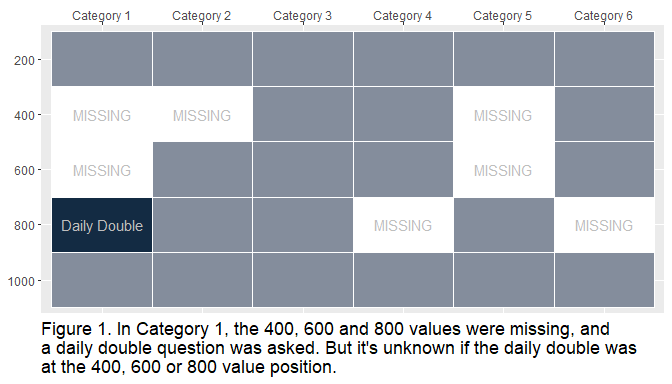
\includegraphics{final_report_files/figure-latex/unnamed-chunk-2-1.pdf}

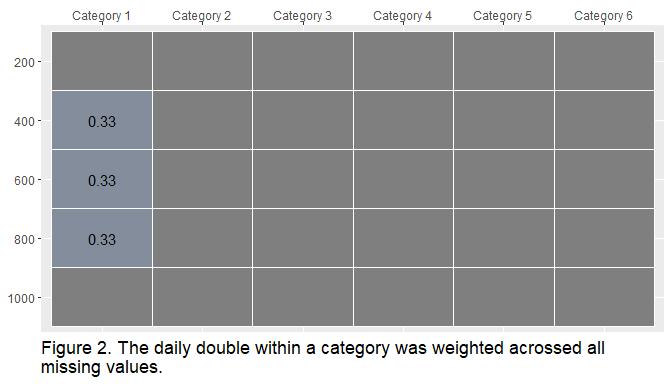
\includegraphics{final_report_files/figure-latex/unnamed-chunk-3-1.pdf}

\hypertarget{results}{%
\subsection{Results}\label{results}}

What did you find out? Most of these slides should be figures or tables.
Discuss your interpretation of your results as you present them.
Ideally, you should be able to show your main results in about 3 slides,
with one figure or table per slide.

The heatmaps for all years, separated by rounds, displays interesting
results. In round 1, the daily double most often occurs in category 1,
point value 800 (7.33\%). Other ``hot'' points are category 4, value 800
(6.81\%) and category 1, value 1000 (6.75\%). The least likely
placements are across all categories in value 100 (0.35\% or less) and
in categories 2 (4.63\% or less) and 6 (4.27\% or less). Value 800 is
favored across all categories (4.27\% -- 7.33\%). In round 2, the daily
double is most often located in category 1, value 1600 (7.06\%). The
other common positions are category 5, value 1600 (6.59\%) and category
3, value 1600 (6.41\%). The least likely occurrences are across value
100 (0.51\% or less) and down category 2 (4.78\% or less) and category 6
(4.75\% or less). Value 1600 is elected for the position most often
across categories (4.75\% -- 7.06\%). Overall, the occurrence of the
daily double remains extremely similar across round 1 and round 2 for
the years analyzed. These results are visually presented in Figure 3
(round 1) and Figure 4 (round 2).

As a secondary question, the heatmaps for all data (rounds 1 and 2) were
faceted by year to look at changes over time. Since the rounds were
similar in the initail analysis, the data was not seperated by round.
The results for years 2001 - 2015 look similar to the results by round.
The ``hot'' points are similar as well as the overall pattern. In 2016,
there seems to be a shift away from the traditional spots. Previously,
catergory 2 was one of the least likely columns but after 2016 the
percentage surpassed the percentages in catergory 1 (previosuly, the
most likely column). There also seems to be a shift from row 4 to row 3.
Before 2016, rows 4 and 5 were the most likely to contain a Daily
Double. After 2016, row 3 a higher percentage of Daily Doubles. The
pattern after 2016 also seems to have more randomness than prior to
2016.

\includegraphics{final_report_files/figure-latex/Daily Doubles by Round-1.pdf}
Figure 3. Percent of Daily Doubles by Position in Round 1\\
~\\
~\\
~\\
\includegraphics{final_report_files/figure-latex/unnamed-chunk-5-1.pdf}
Figure 4. Percent of Daily Doubles by Position in Round 2\\
~\\
~\\
~\\
\includegraphics{final_report_files/figure-latex/Daily Double Heatmap by year-1.pdf}
Figure 5. Percent of Daily Doubles by Position Faceted by Year\\
~\\
~\\
~\\
\#\# Conclusions

The results of this analysis are very similar to previous analyses on
Daily Double location by round. One of the original analyses of Daily
Double location was conducted by Nathan Yau
(\url{https://flowingdata.com/2015/03/03/where-to-find-jeopardy-daily-doubles/})
in 2015. The results of this study look similar to his heatmap that
shows the location of all Daily Doubles for 31 seasons. Yau's analysis
was done because of a Jeopardy contestant, Arthur Chu, that appeared on
the show in 2014. Arthur Chu found success on the show by jumping around
the board hunting for the Daily Doubles. He was not the first to adopt
this strategy, but was one of the most controversial players because of
his approach. Since 2015, there have been other analyses that looked at
the same question and found similar results by round. To our knowledge,
no other analyses have look at the data by year. This analysis included
data up to 2019 and showed a noticable shift in location around
2015/2016. This shift likely occured because of Arthur Chu and the
subsequent analyses of Daily Double locations. This change should be
analyzed over the next few years to see if another pattern is
established or if Jeopardy adopts a more random Daily Double placement.


\end{document}
